\section{Sub-Threshold Logic}
\label{sec:subthresh}

\subsection{Design}
Sub-threshold logic works by reducing the supply voltage to below the threshold voltage of the transistors.
This uses the leakage current from gate to source as the switching current in the device \cite{ULPSubThresh}.
The main form of current flow in the transistor is the current flowing between the drain and the source.
In subthreshold systems the transistor is in very weak inversion, which means that the channel between the drain and source which is normally open in standard CMOS logic is closed off.
This results in a fraction of the normal current flow than would normally be experienced, this is the `leakage' current.
As the leakage current is exponentially related to the gate voltage, reducing the voltage to below the devices threshold voltage results in the leakage current being greatly reduced.
The knock-on effect of this is an exponential increase in delay can be expected.

The increase in the delay makes subthreshold logic very good for applications which require bursts of computation, spread out over a long period of time.
An example of this can be seen in figure \ref{fig:burstST}.
The upper waveform shows the activity status of a standard CMOS logic gate operating in bursts, when the waveform is at the high level the transistor is active and when the waveform shows low the transistor is inactive.
The lower waveform relates to the activity of a subthreshold circuit.
Under these conditions the standard CMOS logic operates over a time $T$, in this way it rapidly completes the computation and then sits idle, until time $T'$ has passed at which point the computation begins again.
The subthreshold logic, needing longer to complete the calculation, is slowed to take the entirety of $T'$ to complete.
As such it achieves a large power reduction while providing the same throughput as its standard CMOS equivalent \cite{IEEEVLSIRobustSTL,ULPSubThresh}.

\begin{figure}
	\centering
	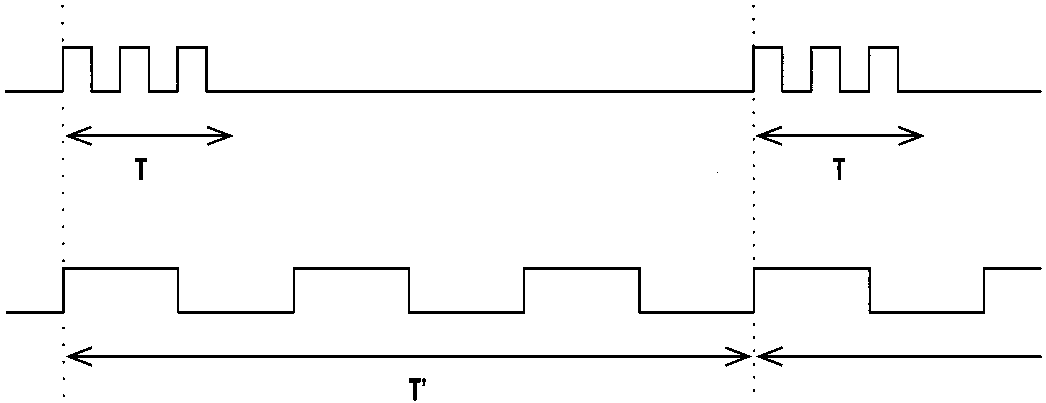
\includegraphics[width=\columnwidth]{../../images/burstycomputation.png}
	\caption{Bursty computation and its relevance to subthreshold operation \cite{IEEEVLSIRobustSTL}}
	\label{fig:burstST}
\end{figure}

In addition to the power saving there are a number of other advantages that subthreshold logic gives.
One of these is an increase in the transconductance gain $gm$ of the device.
Under subthreshold operation the relationship between $V_{gs}$, the voltage across the gate and source, and $I_{ds}$, the current between drain and source, becomes exponential \cite{ULPSubThresh}.
As transconductance gain is defined as $gm = \frac{I_{ds}}{V_{gs}}$, the exponential relationship results in the transconductance gain becoming very large.
Additionally the static noise margin of the device is improved to almost ideal levels.

Furthermore, there are some additional costs in order to achieve the desired power savings.
The devices sensitivity to the temperature, process variations, and power supply noise increases.
As shown in figure \ref{fig:VgsIds} as $V_{gs}$ increases so does the current $I_{ds}$, however the device then enters saturation region at which point $I_{ds}$ levels out.
In this mode of operation, when there is variation on the power supply $V_{gs}$ also varies, however there is minimal change in $I_{ds}$.
With subthreshold logic, the device is operating in the triode region where a change in $V_{gs}$ results in a large change in $I_{ds}$, as such the transconductance gain with respect to the power supply has increased.

\begin{figure}
	\centering
	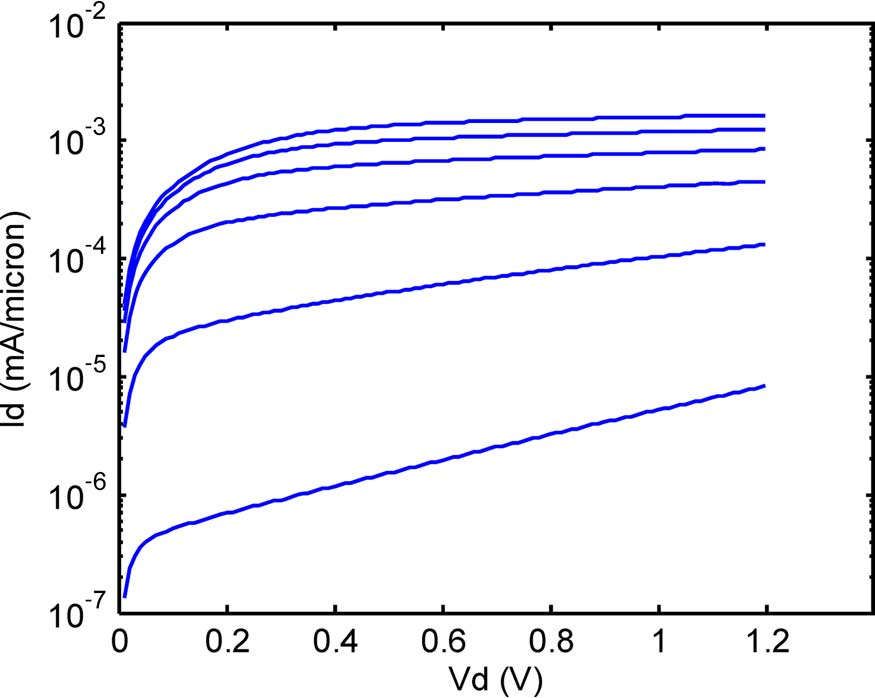
\includegraphics[width=\columnwidth]{../../images/vgsvsids.png}
	\caption{$V_{gs}$ vs. $I_{ds}$ \cite{SemiEmpiricalModels}}
	\label{fig:VgsIds}
\end{figure}

\subsection{Variations}
\subsubsection{Variable Voltage}
In \cite{IEEEVLSIRobustSTL} \citeauthor{IEEEVLSIRobustSTL} attempt to improve subthreshold designs so that they are less susceptible to a number of the side effects experienced in standard subthreshold operation.
Variable Voltage Subthreshold CMOS (VT-Sub-CMOS) logic is an attempt to reduce the effect of temperature and process variations.

VT-Sub-CMOS works by having a stabilisation circuit involved which adjusts the bias applied to the substrate of the transistors, as shown in figure \ref{fig:vtsubcmos}.
This stabilisation circuit consists of two key parts, the leakage current monitor, and the self-substrate bias.
The leakage current monitor acts like a current sensor, and monitors the amount of leakage current flowing through the transistor.
An output voltage is produced which is then passed into the self-substrate bias.
The self-substrate bias then determines an appropriate bias voltage to apply to the substrates.
As this bias voltage then corrects the leakage current a closed loop is formed and the circuit is held stable.

The stabilisation circuitry relies on the basis that the temperature and process variations will be fairly constant across the device, or at least across a small area.
To form the leakage current monitor a transistor is placed in series with a resistance, and the two are then connected between the two power rails, with the gate of the transistor connected to the appropriate power rail to bring it into saturation.
An output voltage is then taken from the centre point of the potential divider that is formed, which is then fed into the self-substrate bias block.
The NMOS and PMOS transistors require separate leakage current mirrors, and hence separate stabilisation circuitry, as production of the two transistor types vary and hence they may experience different process variations.
The self-substrate bias then contains a ring oscillator with an enable controlled by the leakage current monitor's output.
The output of this ring oscillator operates a charge pump which builds a charge on the substrates.
As such this stabilisation circuitry acts to rebuild the charge whenever it falls below a defined value.

SPICE simulations show that this VT-Sub-CMOS logic stays stable as the temperature changes \cite{IEEEVLSIRobustSTL}, effectively bringing the threshold voltage down to just below the supply voltage.
This removes the exponential relationship between $V_{gs}$ and $I_{ds}$, reducing the sensitivity to temperature variations.
The delay required between switching is also greatly reduced, meaning that the system can operate at a higher frequency.
While this approach introduces stability into the subthreshold logic, it increases the circuit complexity, and hence also increases the area.

\begin{figure}
	\centering
	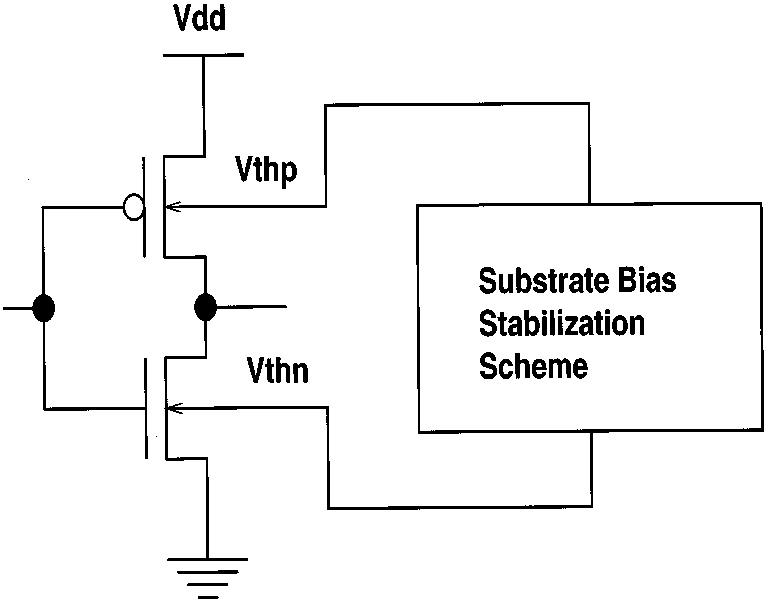
\includegraphics[width=\columnwidth]{../../images/vtsubcmos.png}
	\caption{The stabilisation scheme used in VT-Sub-CMOS \cite{IEEEVLSIRobustSTL}}
	\label{fig:vtsubcmos}
\end{figure}

\subsubsection{Dynamic Voltage}

